\section{Experimentation}
\subsection{Data Augmentation}
\noindent
Data augmentation is performed on images of the hand and upper body poses to reduce the model overfitting. This helps in generalising on a variety of poses better. Table \ref{table:augmentation_step} shows the augmentation steps performed on the poses and images. Flipping and mirroring is not performed for the upper body pose since the upper body is symmetric to some extent. All the joints of the hand and body pose are within the image after rotation and translation.

\begin{table}[ht]
\centering
\begin{tabular*}{\textwidth}{c @{\extracolsep{\fill}} p{2.5in} cc}
\hline
Augmentation Step & \centering Description & Hand Pose & Upper Body Pose \\ [0.5ex] 
\hline
Brightness & Adjusted image brightness by a factor in the range of [-0.25, 0.25] & Yes & Yes \\ 
Contrast & Adjusted image contrast by a factor in the range of [-0.25, 0.25] & Yes & Yes  \\
Sharpness & Adjusted image sharpness by a factor in the range of [-0.25, 0.25] & Yes & Yes \\
Mirror & Mirror original image & Yes & No \\
Flip & Flip original image & Yes & No \\
Rotate & Rotate by an angle in the range of [0, 360) degrees & Yes & Yes \\
Translate & Translate by a pixel in the range of [-100, 100] pixels & Yes & Yes  \\ 
Fill holes & Fill black pixels after transformation with background images & Yes & Yes  \\ 
[1ex] 
\hline
\end{tabular*}
\caption{Augmentation Steps}
\label{table:augmentation_step}
\end{table}
\noindent
The rotation step in the data augmentation is given in Equation \ref{eq:rotation_data_augmentation}. The rotation matrix is applied on the 3D keypoints to rotate the 3D pose and 2D pose about the z-axis.
\begin{equation}
\mathbf{P_{rotated}} = \begin{bmatrix}
cos(\theta) & -sin(\theta) & 0\\
sin(\theta) & cos(\theta) & 0\\
0 & 0 & 1
\end{bmatrix}
\mathbf{P}\label{eq:rotation_data_augmentation}
\end{equation}
\noindent
The translation step in the data augmentation is given in Equation \ref{eq:translation_x_data_augmentation} and \ref{eq:translation_y_data_augmentation}. \(p_{x}\) and \(p_{y}\) refers to the translation of 2D keypoints in the image and is measured in pixels. Similar triangles is applied to compute the translation of 3D keypoints.
\begin{equation}
x_{new} = x_{old} - \frac{p_x}{f_x} \times z \label{eq:translation_x_data_augmentation}
\end{equation}
\begin{equation}
y_{new} = y_{old} - \frac{p_y}{f_y} \times z \label{eq:translation_y_data_augmentation}
\end{equation}

\newpage
\subsection{Experimented Models}
\noindent
For this project, 4 different models were designed and experimented. The models were then modified to finetune the hyperparameters.

\noindent
The first model follows Chernytska and Zhaos' methods for encoder-decoder architecture of the 2D pose estimation model \cite{olha, semgcn}. A ResNet34 is used as the encoder. Skip connections are used in the decoder to concatenate the image embedding and the decoded information to obtain the heat maps. The 3D pose regressor follows Bazarevsky's high-level architecture \cite{blazepose}; however, the exact architecture is unknown. As a first attempt, each module in the regressor consists of a convolution layer and a residual block. This gives the model the complexity while avoiding the vanishing gradient problem. The heat maps and encoded information of the residual layers provide information to estimate the 3D poses. The last layer is a fully-connected layer and has an output size of 63 for x, y, and z coordinates for the 21 keypoints. The model architecture is shown in Figure \ref{fig:model_v1}.

\begin{figure}[ht]
	\begin{center}
		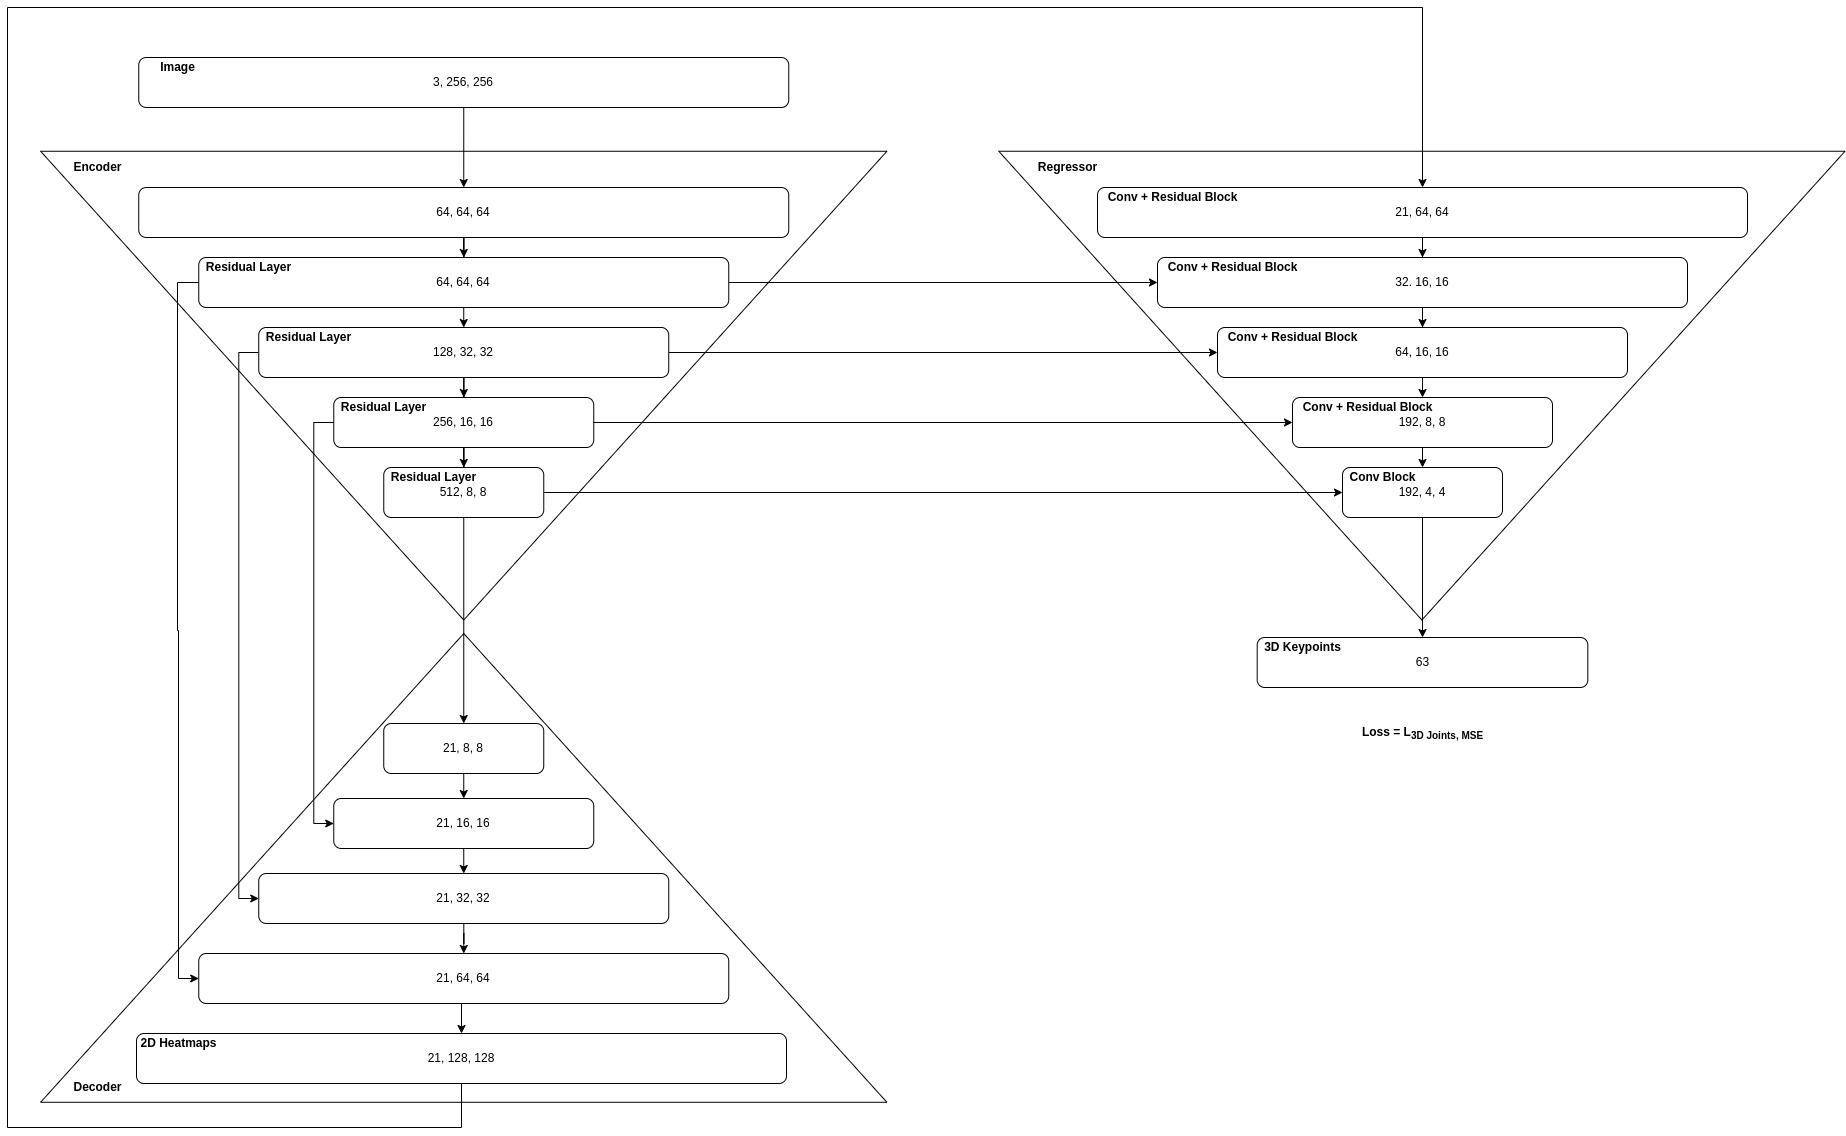
\includegraphics[width=450px]{assets/Model_v1.jpg}
		\caption{Model v1}
		\label{fig:model_v1}
	\end{center}
\end{figure}

\newpage

\noindent
Since this project is concerned with the estimation of 3D poses, the hyperparameters of the regressor model are modified, keeping the encoder-decoder module the same. Figure \ref{fig:model_v1_x} shows 3 different modifications to Model v1. The top left regressor is the original version. The top right regressor removes the heat map layer to determine if the heat map provides any useful information in estimating the 3D poses. The bottom left regressor increases the number of output channels in each layer to determine if more channels can learn better features for the estimation. The bottom right regressor decreases the output channels in each layer instead to determine if the model can still perform with fewer parameters.

\begin{figure}[ht]
	\begin{center}
		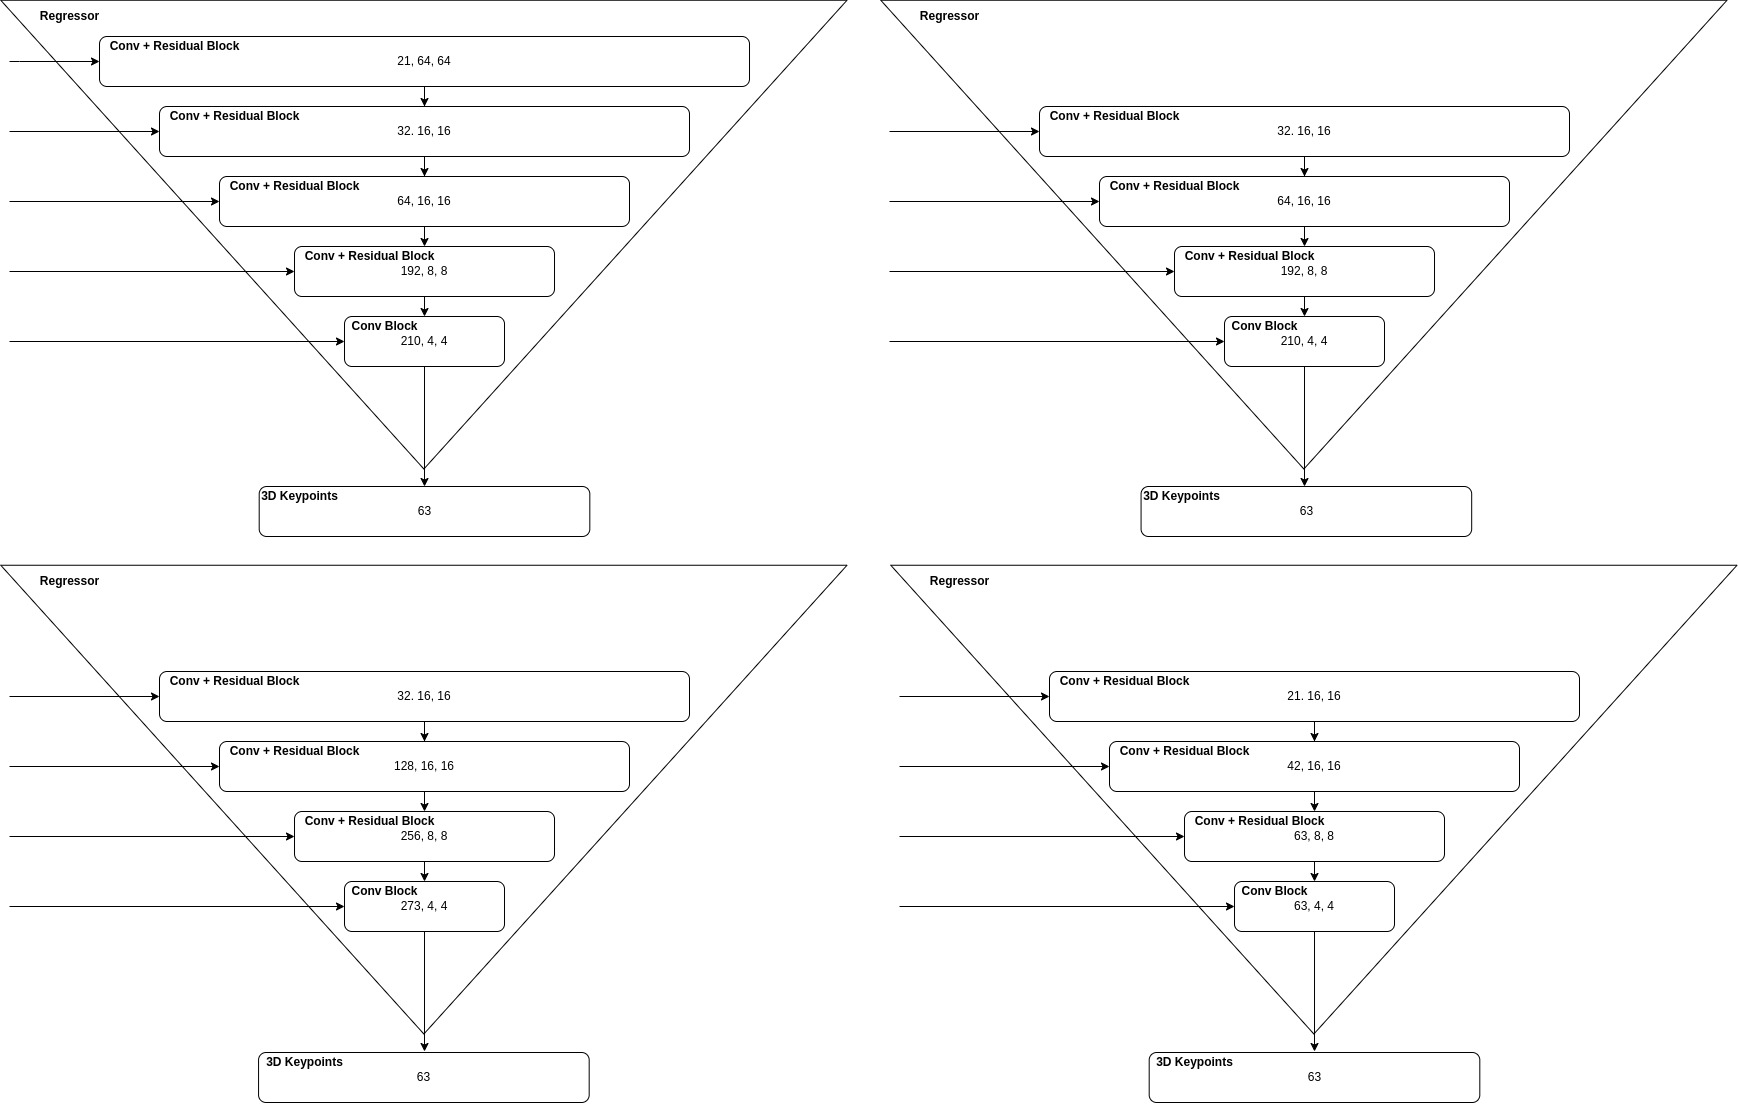
\includegraphics[width=450px]{assets/Model_v1.x.jpg}
		\caption{Hyperparameter Tuning For Model v1}
		\label{fig:model_v1_x}
	\end{center}
\end{figure}

\newpage

\noindent
The second model designed and experimented uses the same encoder-decoder architecture as the first model. The regressor model in the second model is almost the same as that of the first model except that each module in the regressor is using a convolution layer instead of a convolution layer and a residual block. This regressor model follows more closely with Bazarevsky's model if each stage in regressor model is a convolution layer (excluding the heat map). Similarly, the last layer is a fully-connected layer and has an output size of 63 for x, y, and z coordinates for the 21 keypoints. The model architecture is shown in Figure \ref{fig:model_v2}.

\begin{figure}[ht]
	\begin{center}
		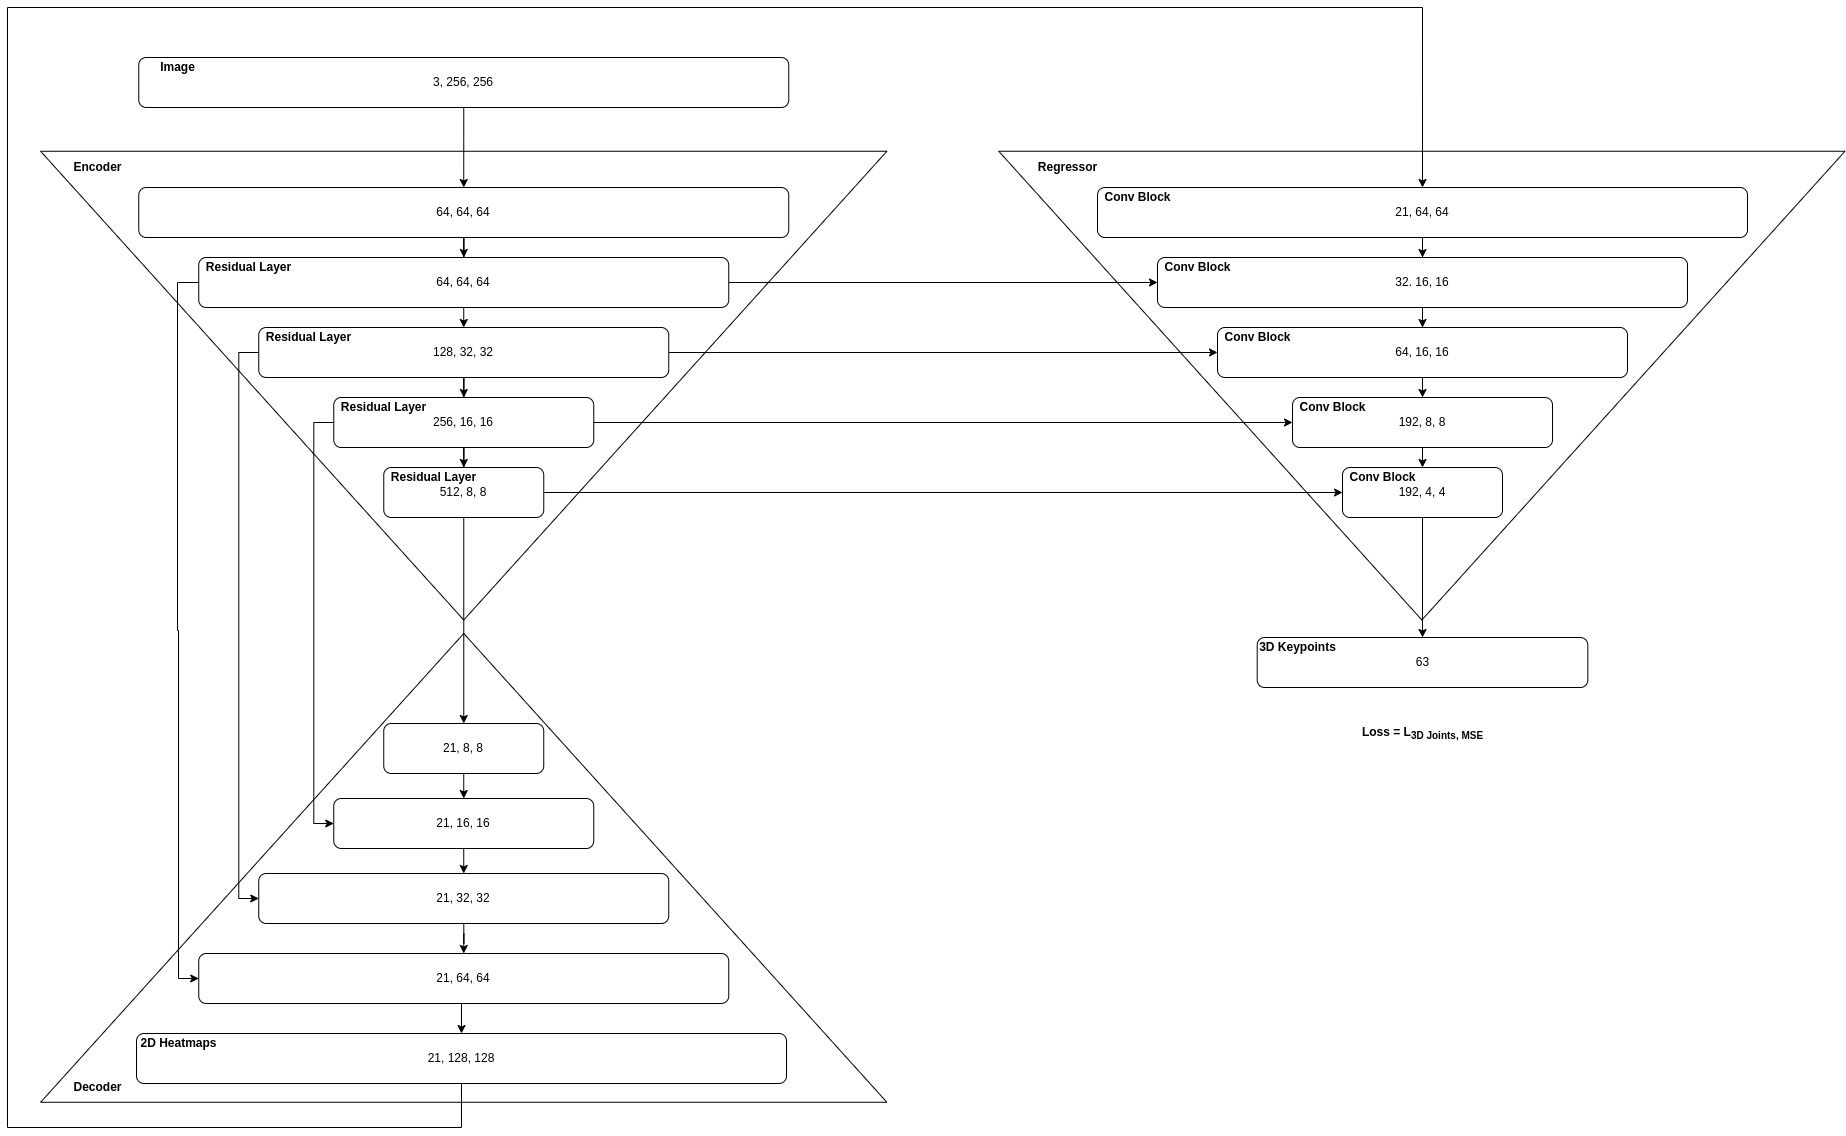
\includegraphics[width=450px]{assets/Model_v2.jpg}
		\caption{Model v2}
		\label{fig:model_v2}
	\end{center}
\end{figure}

\newpage

\noindent
The hyperparameters of the second model are modified, keeping the encoder-decoder modules the same. Figure \ref{fig:model_v2_x} shows 3 different modifications to Model v2. The top left regressor is the original version. The top right regressor removes the heat map layer to similarly determine if the heat map provides any useful information in estimating the 3D poses. The bottom left regressor increases the number of output channels in each layer to similarly determine if more channels can learn better features for the estimation. The bottom right regressor decreases the output channels in each layer instead to similarly determine if the model can still perform with fewer parameters. Like the first model, the same set hyperparameters were modified in the second model to concur the impact on the performance.

\begin{figure}[ht]
	\begin{center}
		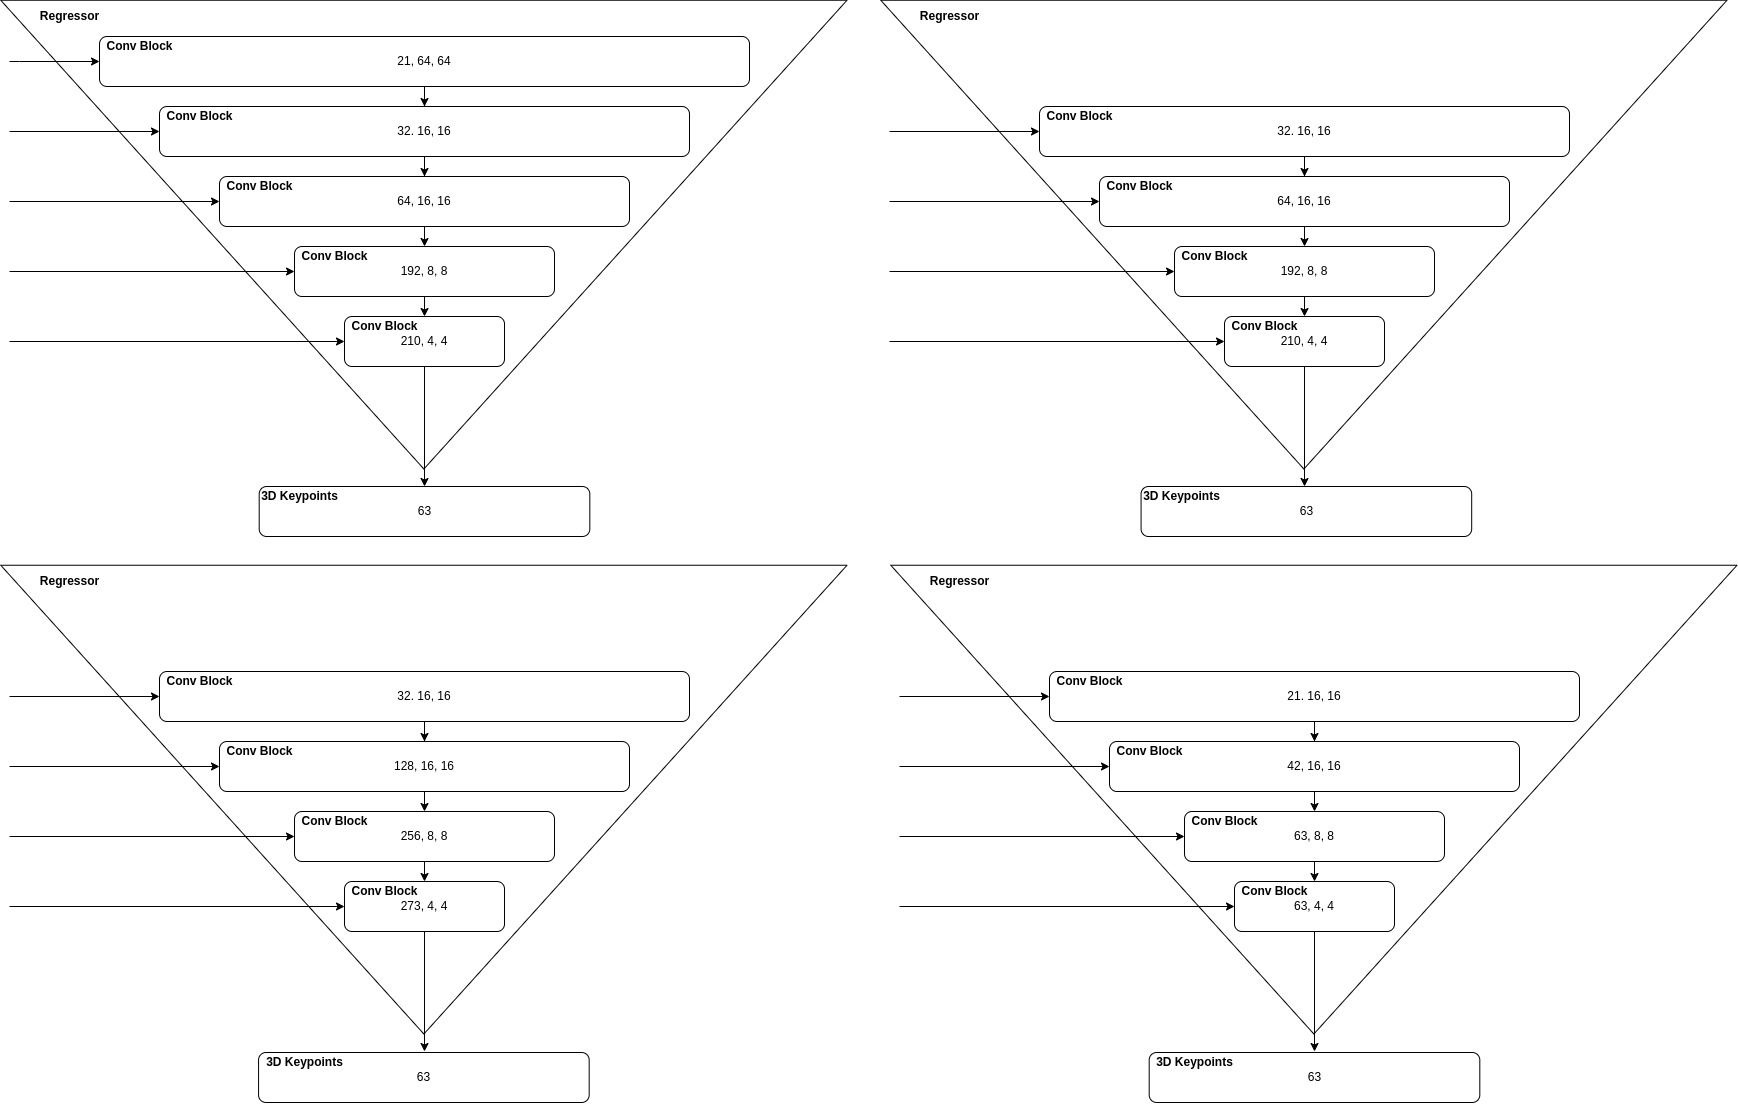
\includegraphics[width=450px]{assets/Model_v2.x.jpg}
		\caption{Hyperparameter Tuning For Model v2}
		\label{fig:model_v2_x}
	\end{center}
\end{figure}

\newpage

\noindent
The third model designed and experimented uses the same encoder-decoder architecture as the first and second model. The third model also used the same regressor model as the second model where each module is a convolution block. Only the final fully-connected layer is replaced with Zhao's SemGCN to estimate the 3D poses \cite{semgcn}. Zhao's proposed a similar architecture, but flatten the image embedding of the residual layers and heat maps as inputs to SemGCN \cite{semgcn}. In this SemGCN, non-local layers are also used to learn the distant relationship between two entities in the graph \cite{semgcn, nonlocal}. The SemGCN layers are repeated 4 times. This model will determine if graph convolution layers give better performance than using a fully-connected layer. The model architecture is shown in Figure \ref{fig:model_v3}. Note that the output channel in the last module of the regressor is different and is a multiple of the number of keypoints to resize to a valid tensor.

\begin{figure}[ht]
	\begin{center}
		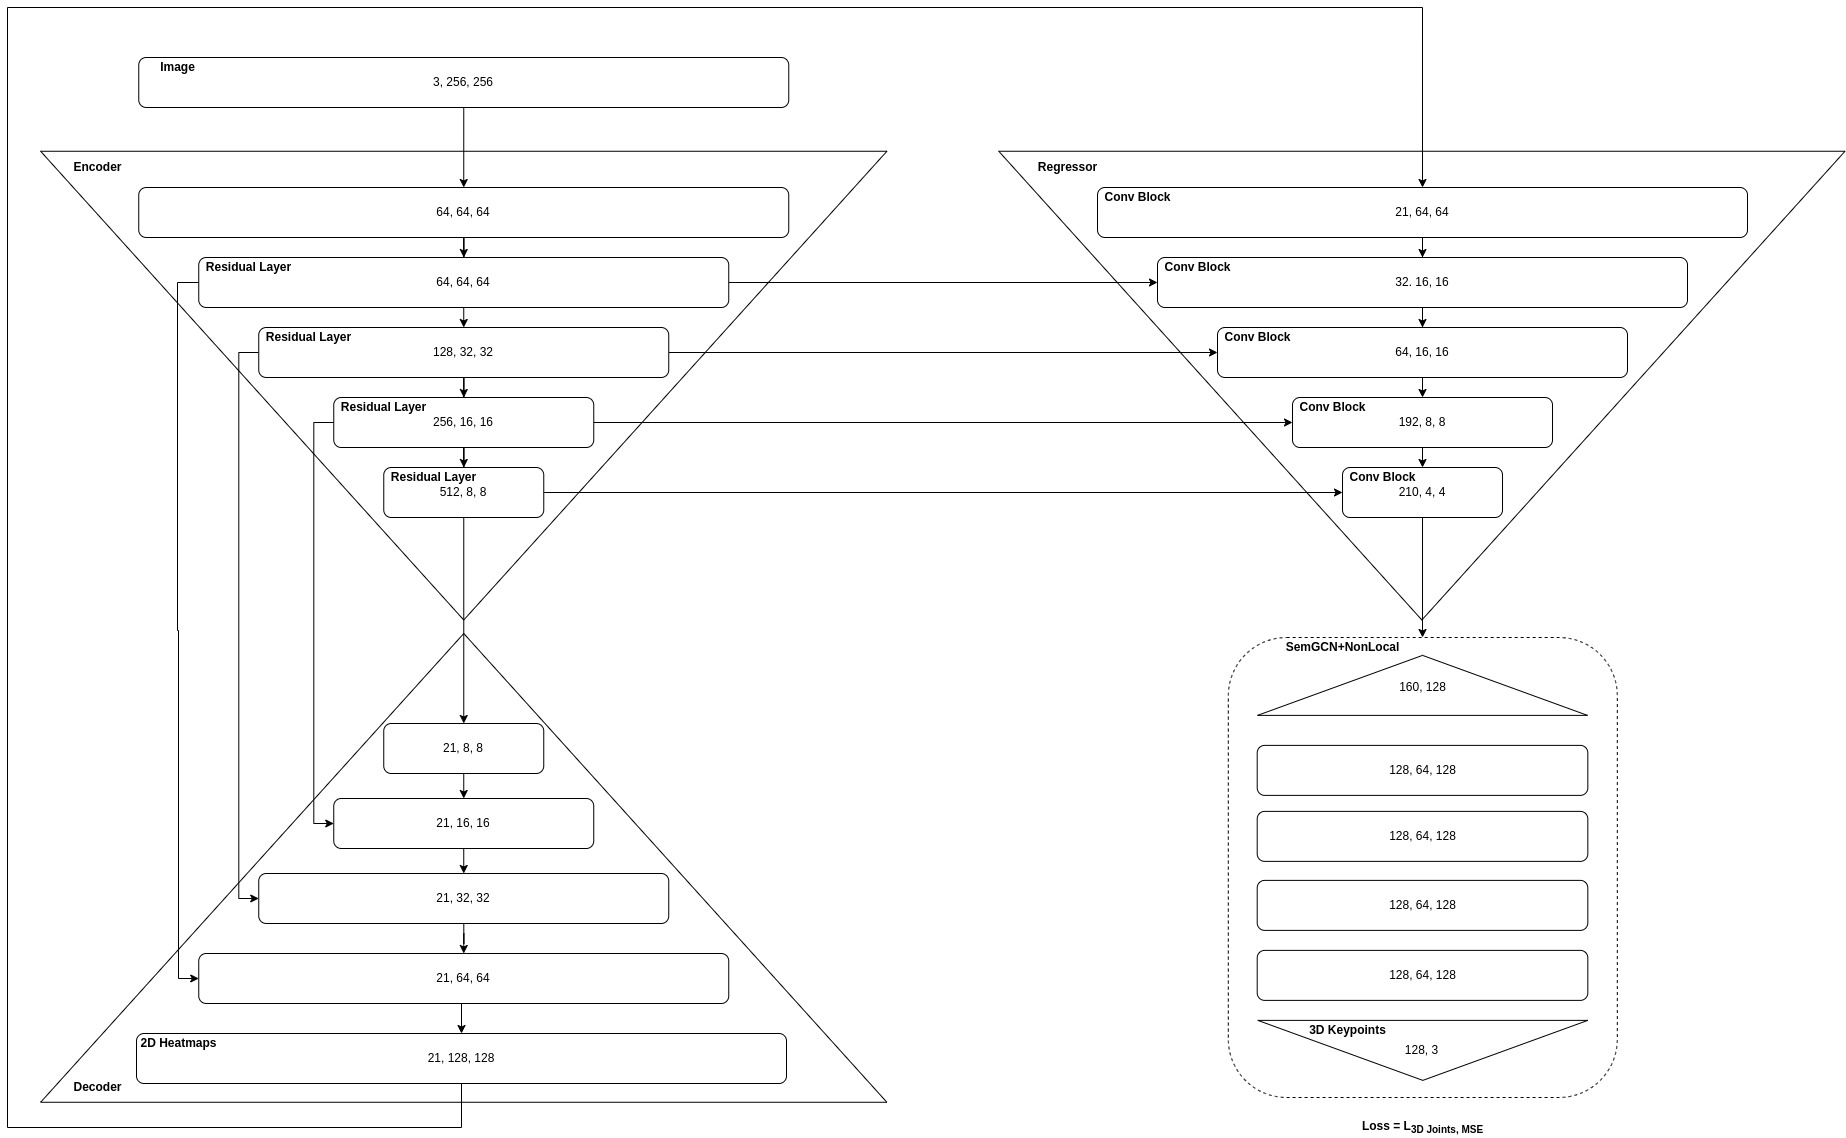
\includegraphics[width=450px]{assets/Model_v3.jpg}
		\caption{Model v3}
		\label{fig:model_v3}
	\end{center}
\end{figure}

\newpage

\noindent
The hyperparameters of the third model are modified, keeping the encoder-decoder module the same. Figure \ref{fig:model_v3_x} shows 3 different modifications to Model v3. The top left regressor is the original version. The top right regressor removes the heat map layer, the bottom left regressor increases the number of output channels in each layer, and the bottom right regressor decreases the output channels in each layer. Like the first and second model, the same set hyperparameters were modified in the third model to concur the impact on the performance.

\begin{figure}[ht]
	\begin{center}
		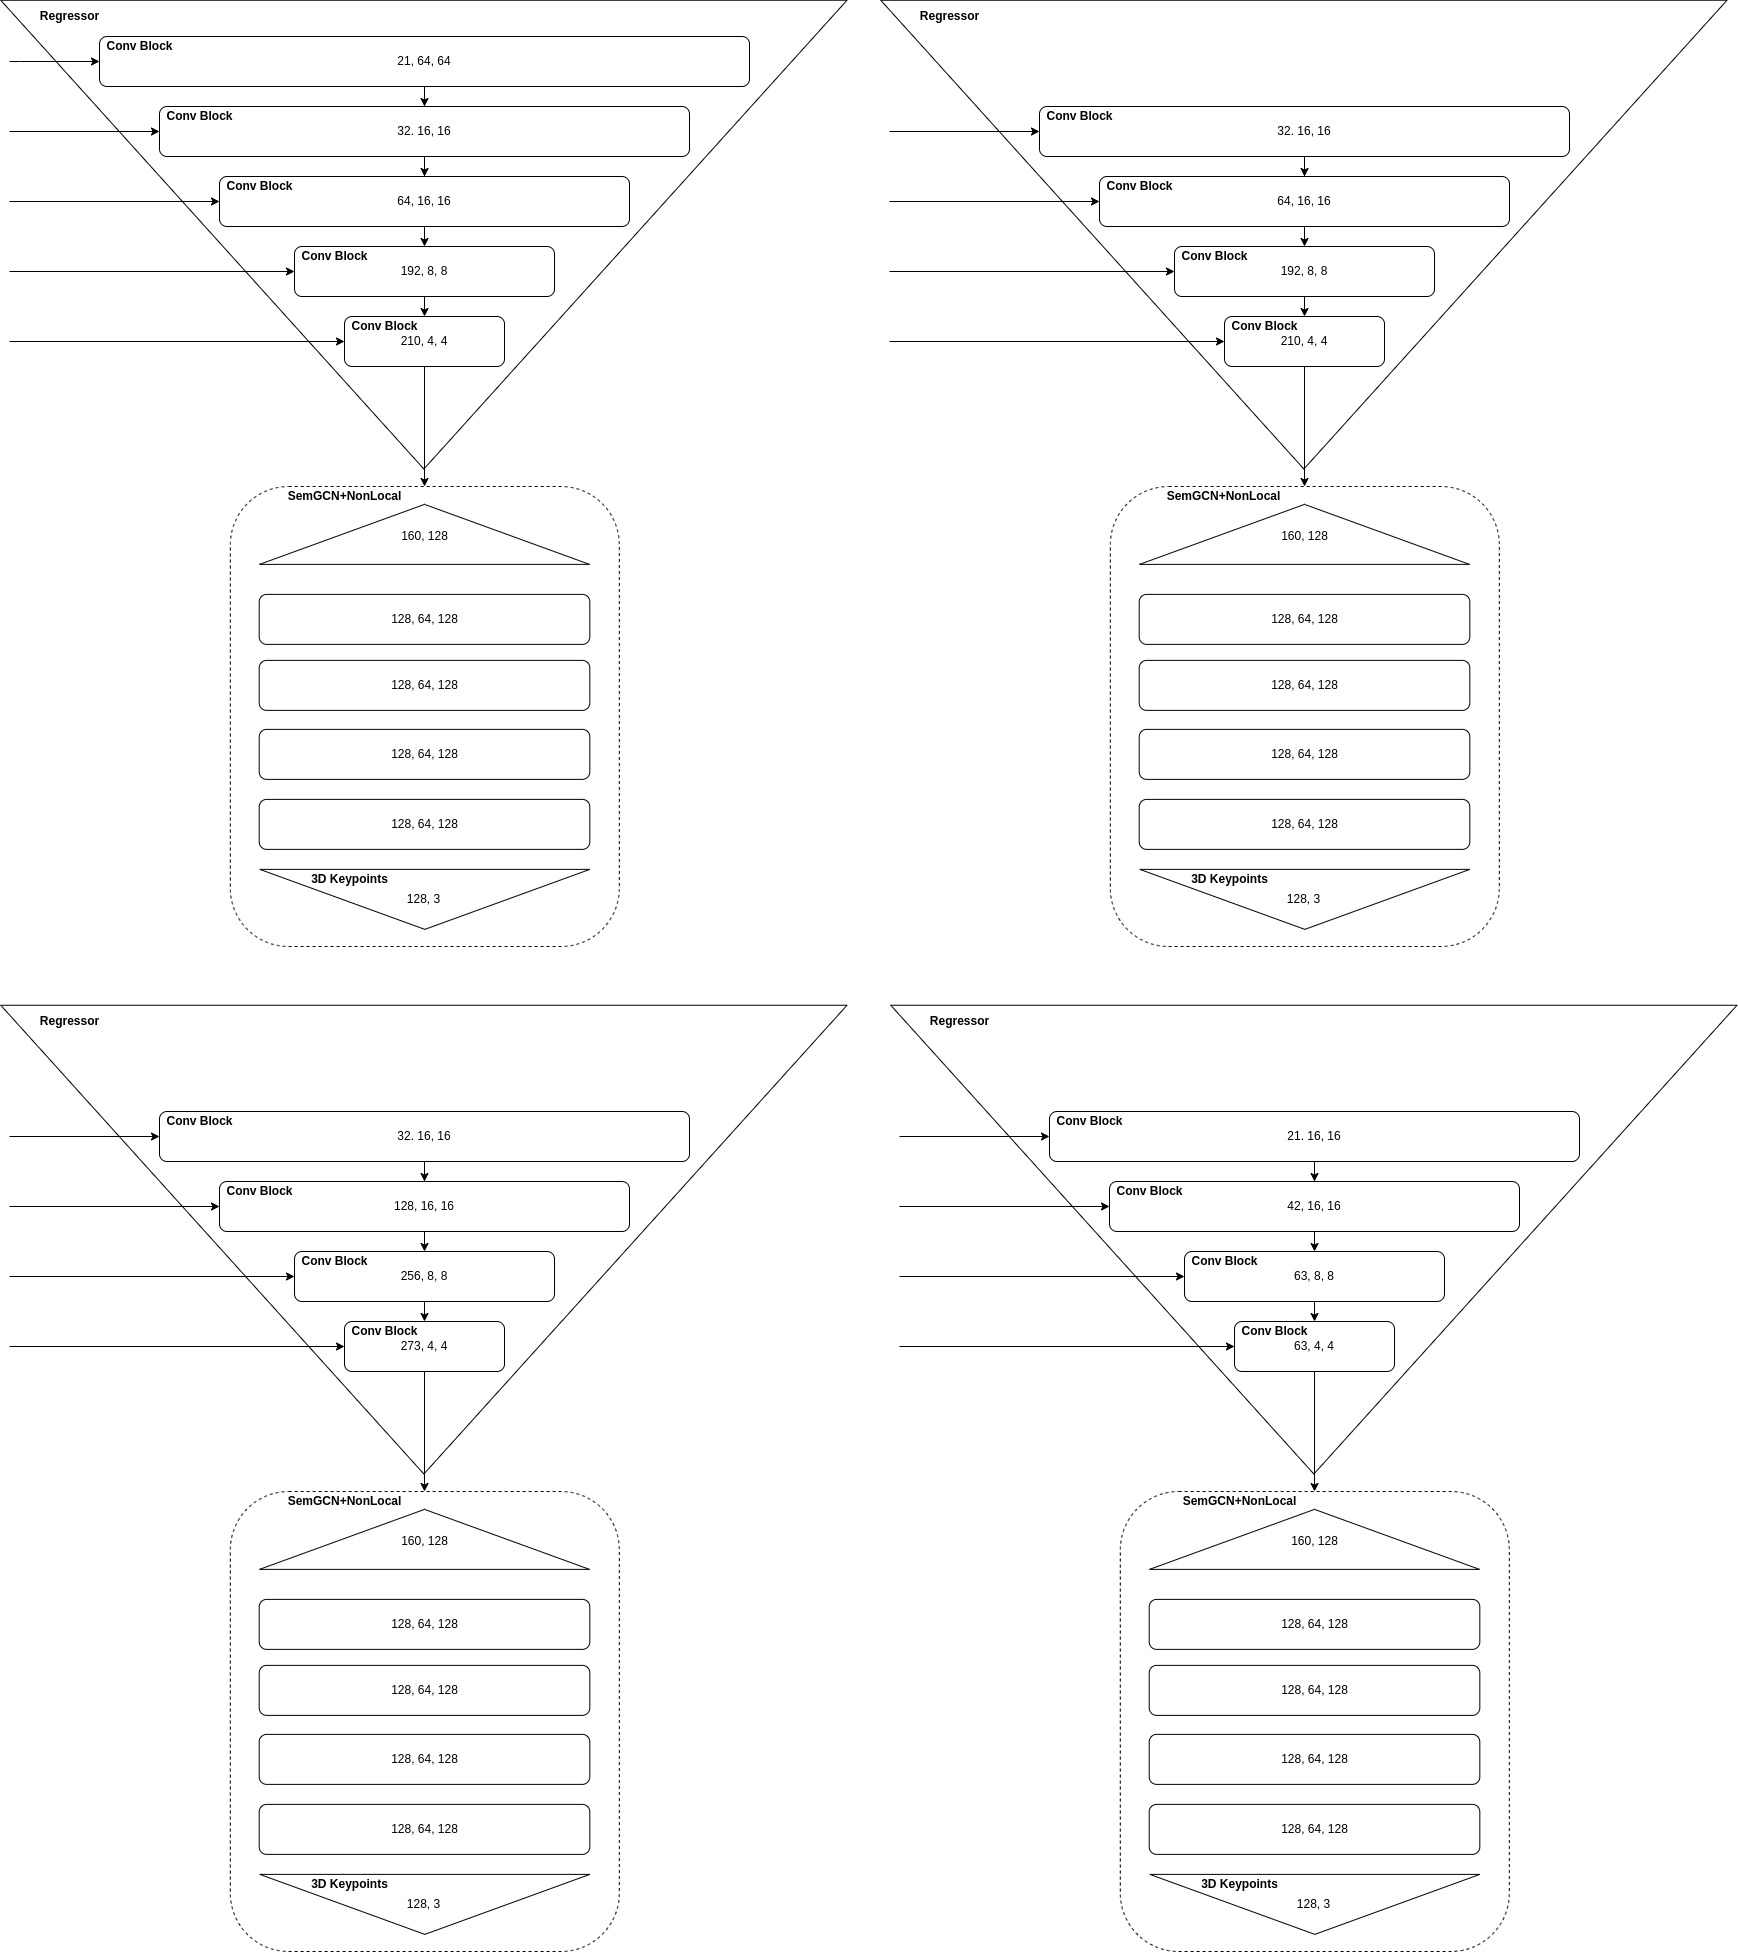
\includegraphics[width=450px]{assets/Model_v3.x.jpg}
		\caption{Hyperparameter Tuning For Model v3}
		\label{fig:model_v3_x}
	\end{center}
\end{figure}

\newpage

\noindent
The fourth model designed and experimented uses the same encoder-decoder architecture as the first, second, and third model. The fourth model also used the same regressor model as the third model where each module is a convolution block and SemGCN layers are used instead of a fully-connected layer. However, non-local layers are not used in this model to determine if the non-local layers can help the model estimate the 3D poses better if distant relationship between two entities in the graph are learnt. The model architecture is shown in Figure \ref{fig:model_v4}.

\begin{figure}[ht]
	\begin{center}
		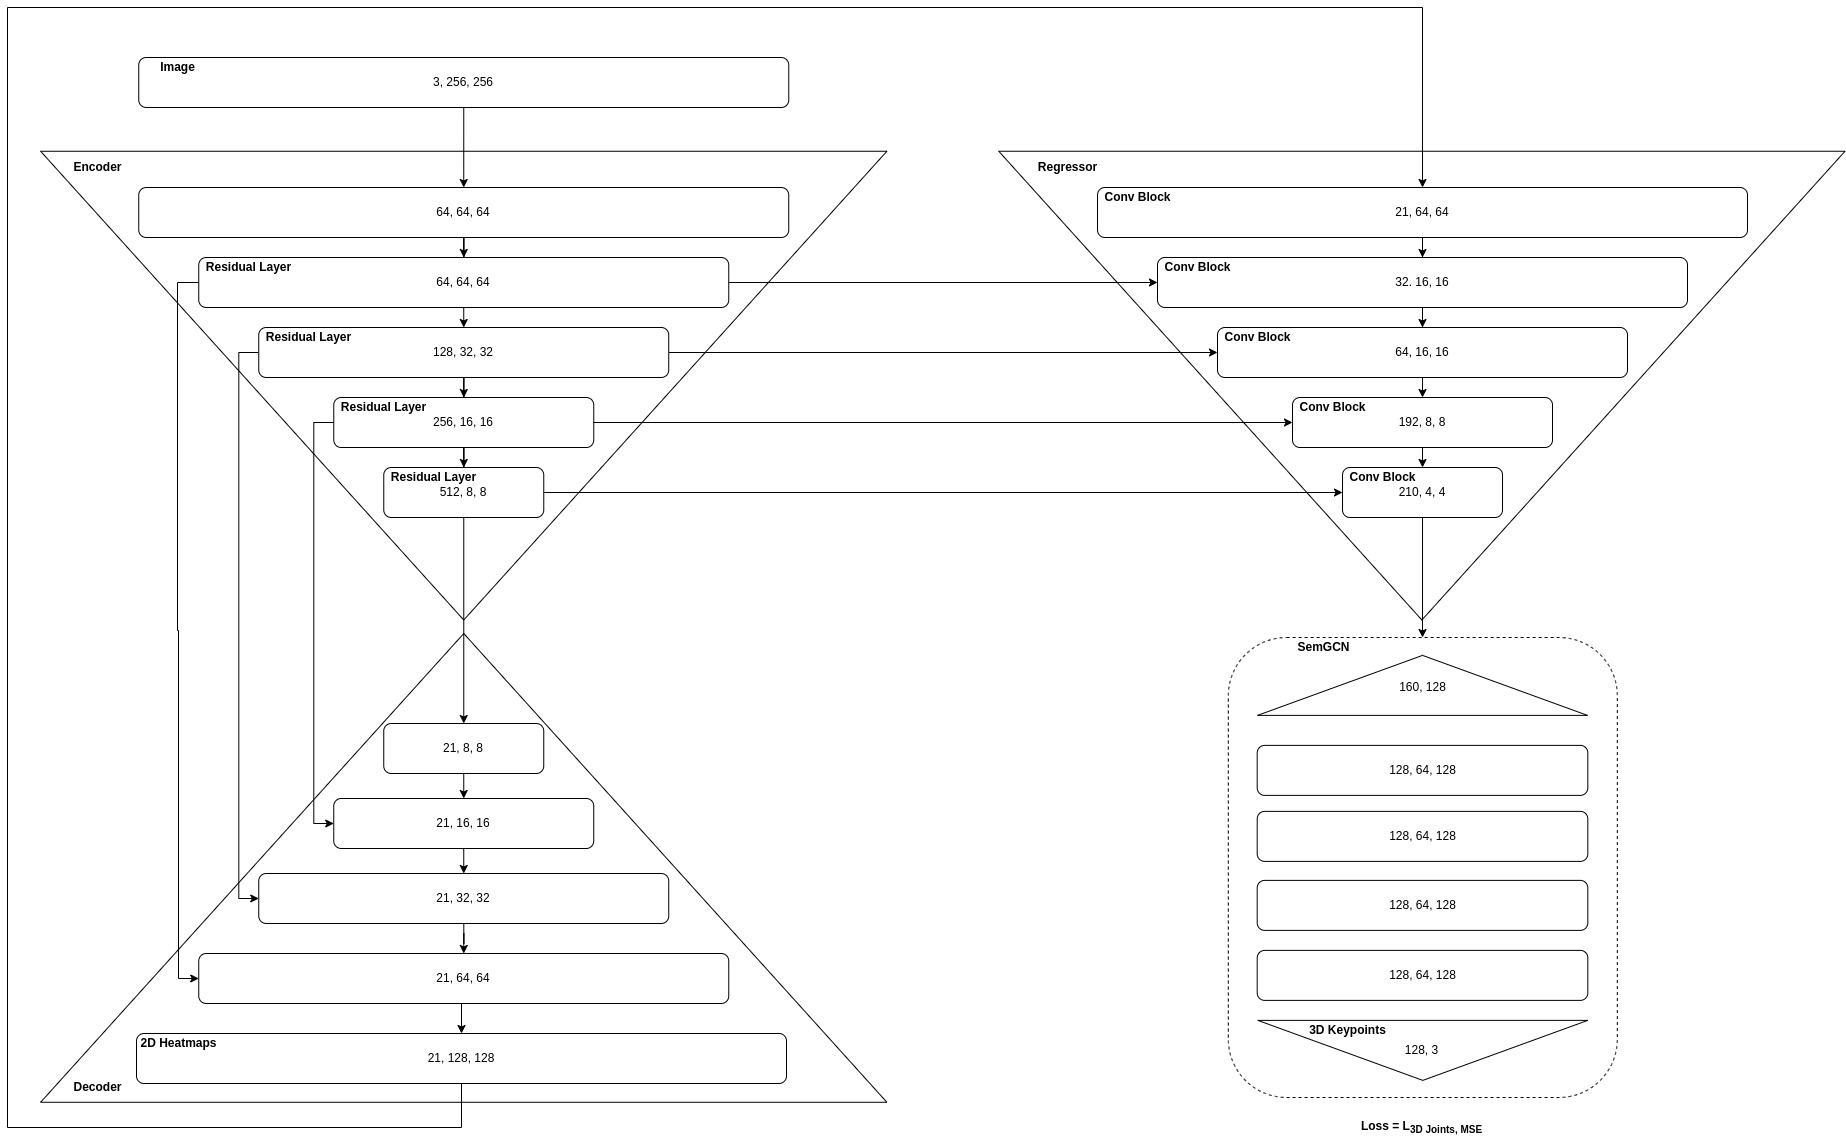
\includegraphics[width=450px]{assets/Model_v4.jpg}
		\caption{Model v4}
		\label{fig:model_v4}
	\end{center}
\end{figure}

\newpage

\noindent
The hyperparameters of the fourth model are modified, keeping the encoder-decoder module the same. Figure \ref{fig:model_v4_x} shows 4 different modifications to Model v4. The top left regressor is the original version. The top right regressor removes the heat map layer, the bottom left regressor increases the number of output channels in each layer, and the bottom right regressor decreases the output channels in each layer. Like the first, second, and third model, the same set hyperparameters were modified in the fourth model to concur the impact on the performance.


\begin{figure}[ht]
	\begin{center}
		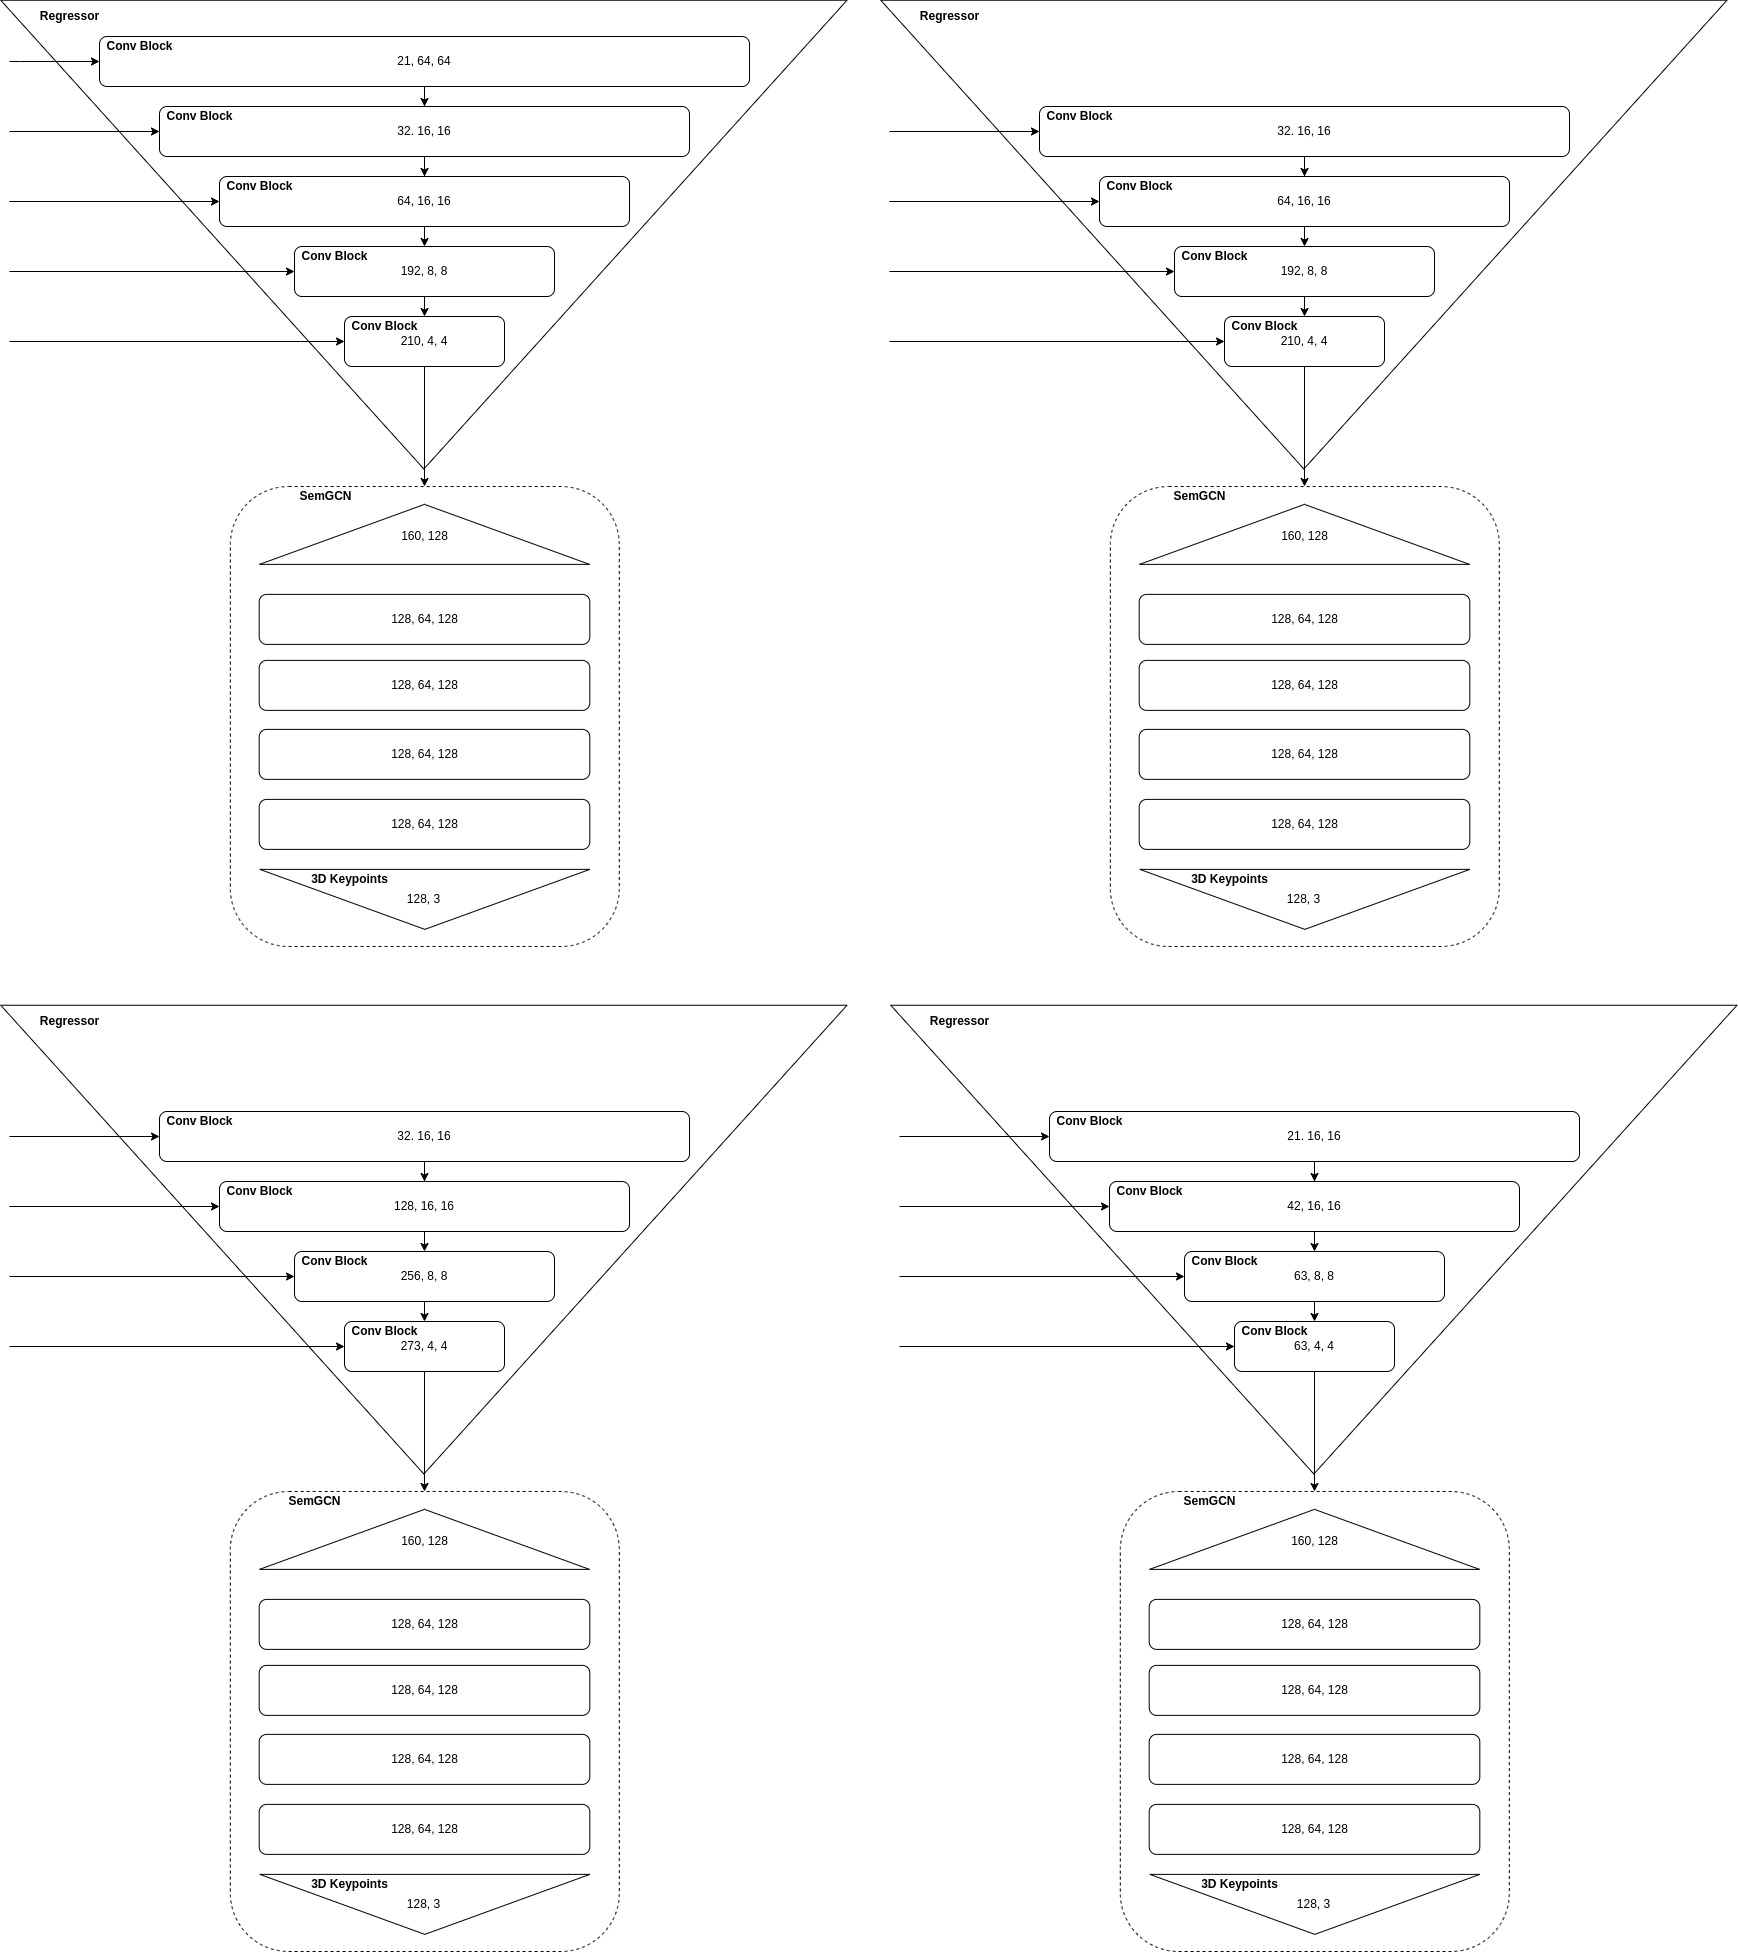
\includegraphics[width=450px]{assets/Model_v4.x.jpg}
		\caption{Hyperparameter Tuning For Model v4}
		\label{fig:model_v4_x}
	\end{center}
\end{figure}

\newpage

\noindent
Later in the results and dicussion, Model v3.1 performed the best and was optimized further. Figure \ref{fig:model_v3_1_x} shows the hyperparameters experimented. The top left regressor used two SemGCN layers and the top middle regressor used 6 SemGCN layers instead of the original 4 layers to understand how the model performs under with more layers and parameters. The top right regressor used two convolution layers instead of one but the output size of the first layer is half of the output size of the second. This reduce the parameters but add depth in the model to determine whether adding layers helps the model learn better than adding channels. The bottom two regressors use additional loss functions. The left regressor is supervised by the MSE of the 2D joints and 3D joints. The right regressor is supervised by the MSE of the 3D joints and 3D bone vector.

\begin{figure}[ht]
	\begin{center}
		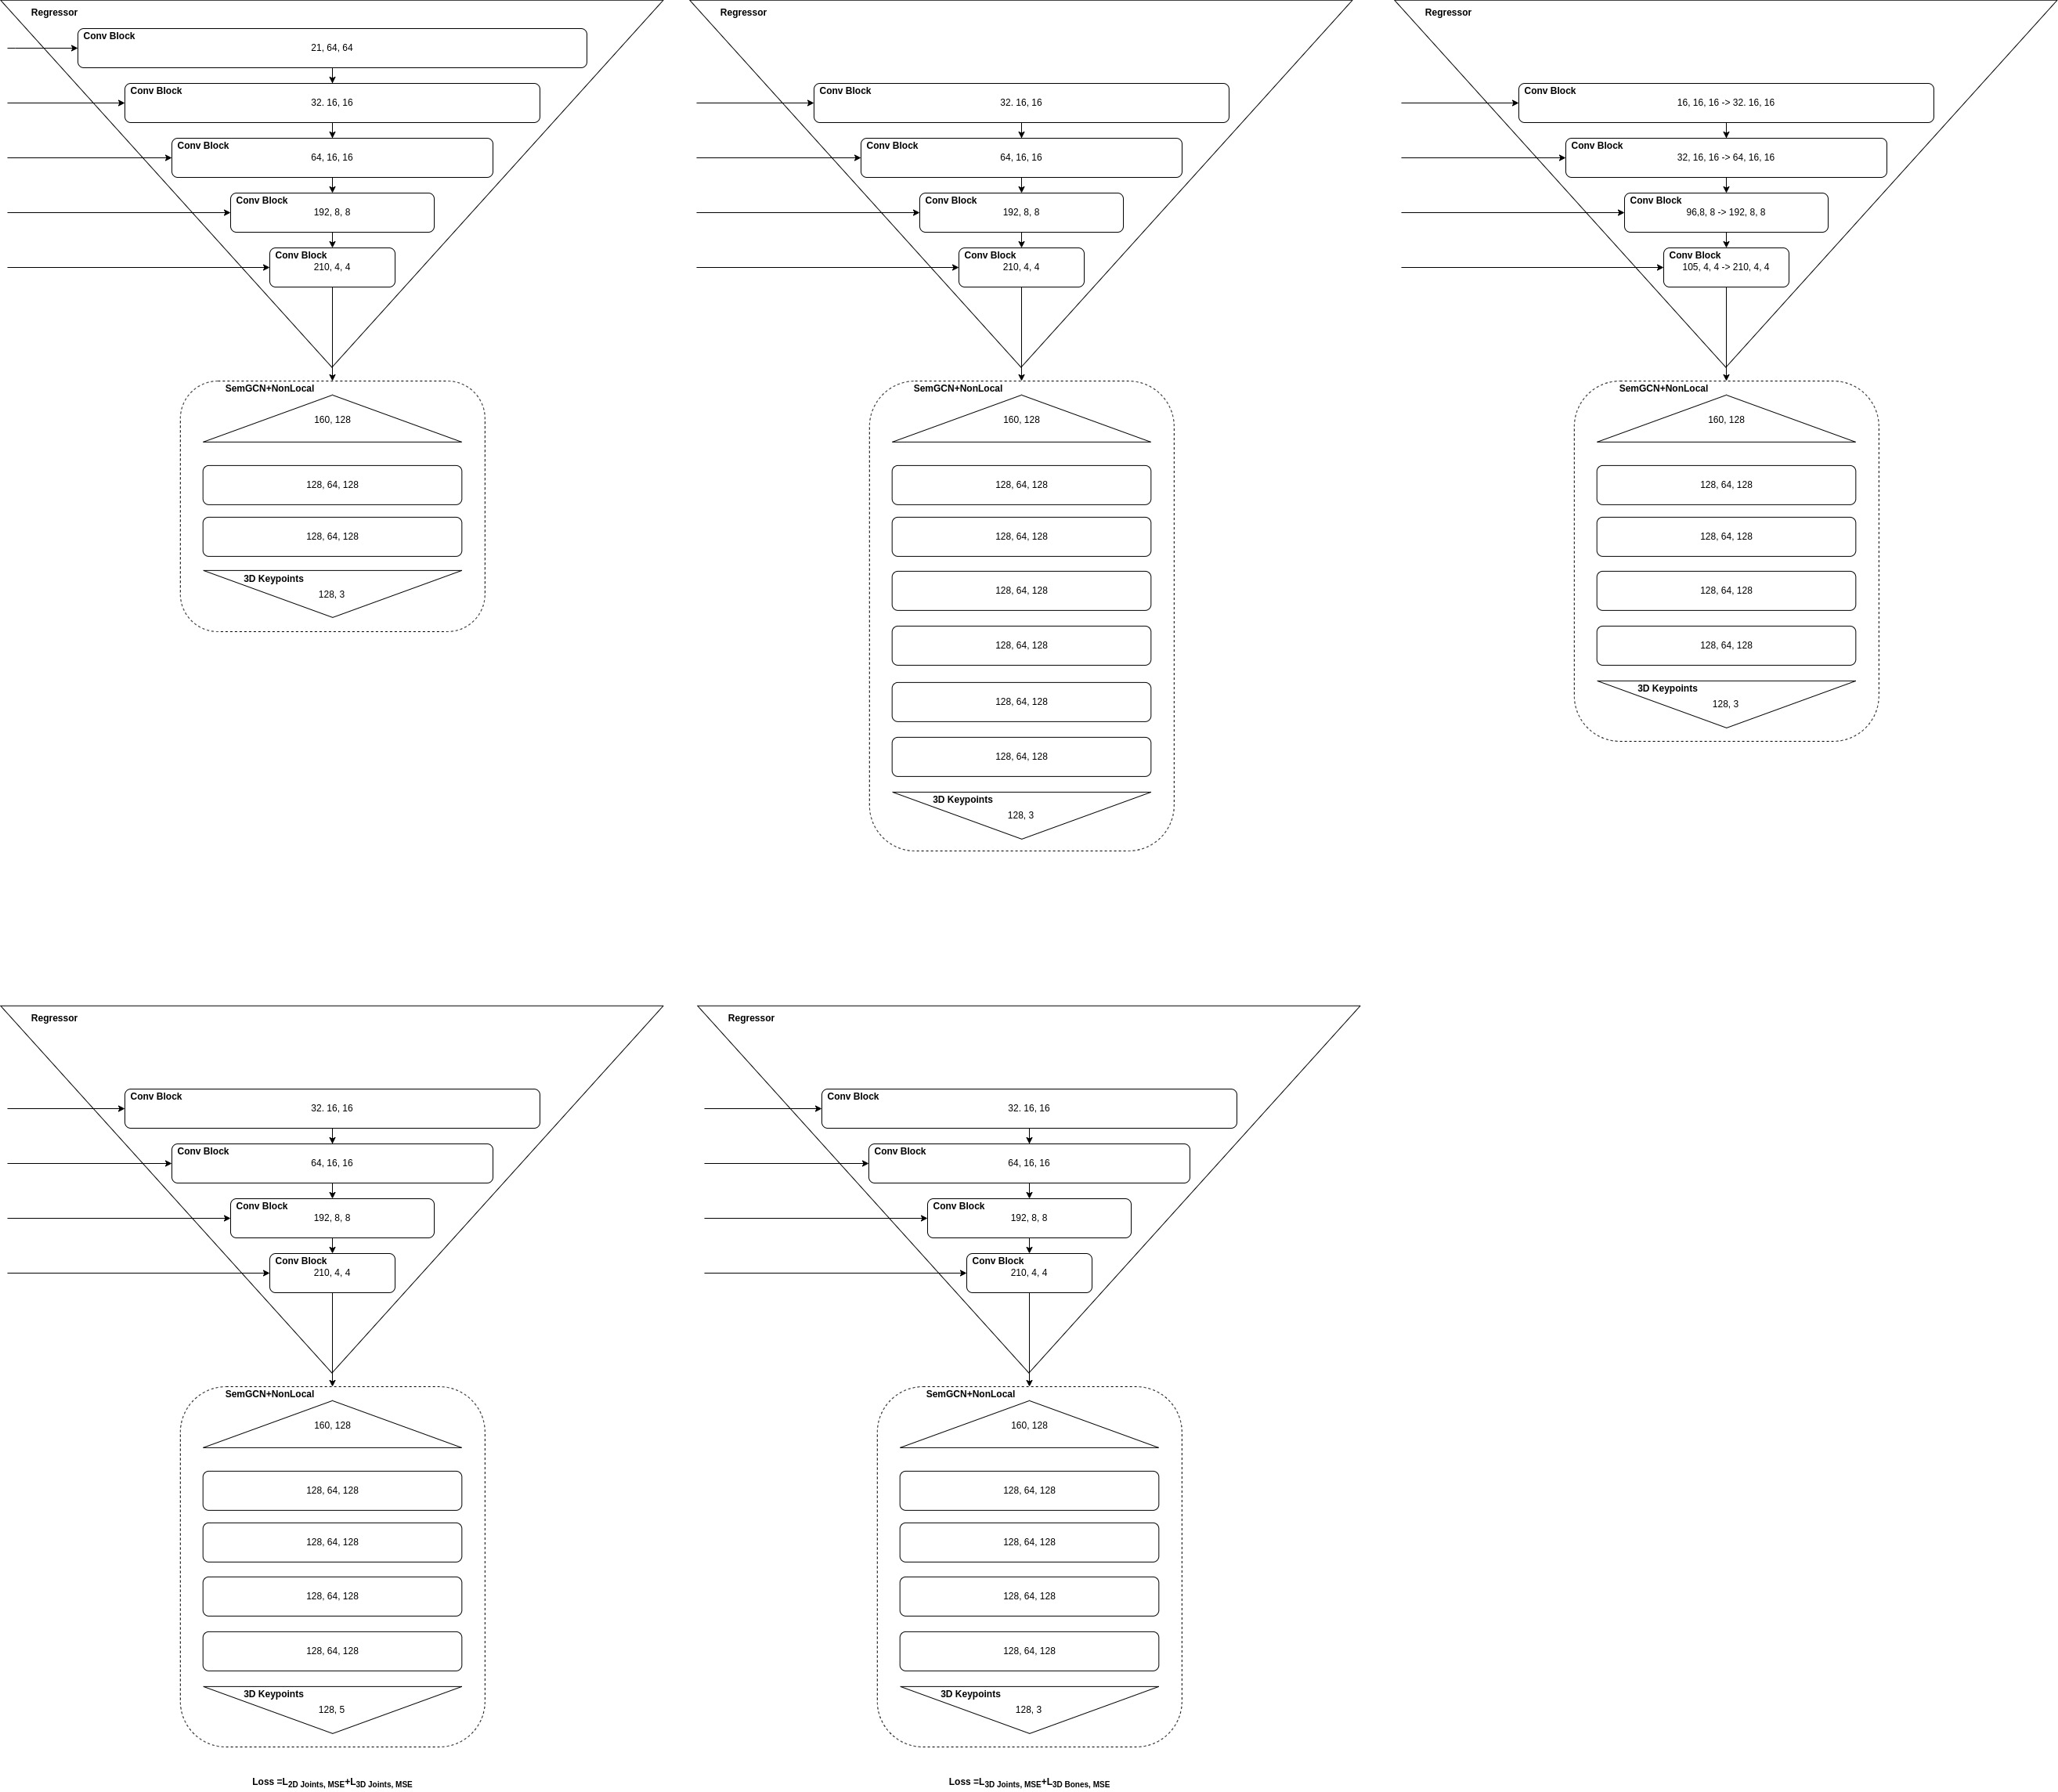
\includegraphics[width=450px]{assets/Model_v3.1.x.jpg}
		\caption{Hyperparameter Tuning For Model v3.1.x}
		\label{fig:model_v3_1_x}
	\end{center}
\end{figure}

\newpage
\noindent
Table \ref{table:model_summary} summarises the different models experimented in this project. The hyperparameters experimented are the heat maps, convolution and regression blocks in the regressor module, SemGCN and fully-connected layer in final layer, and the loss functions. After all the experiments, this project uses v3.1.6 as the final model.

\begin{table}[ht]
\centering
\begin{tabular*}{\textwidth}{c @{\extracolsep{\fill}} cccc}
\hline
Models & Heat map & Regressor Module & Final Layer & MSE Loss Function \\ [0.5ex] 
\hline
v1.0  & Yes & 1 Conv + Residual Block & Fully-Connected & 3D Joints \\
v1.1  & No & 1 Conv + Residual Block & Fully-Connected & 3D Joints \\ 
v1.2  & No & 1 Conv + Residual Block & Fully-Connected & 3D Joints \\ 
v1.3  & No & 1 Conv + Residual Block & Fully-Connected & 3D Joints \\ 
v2.0  & Yes & 1 Conv & Fully-Connected & 3D Joints \\
v2.1  & No & 1 Conv & Fully-Connected & 3D Joints \\ 
v2.2  & No & 1 Conv & Fully-Connected & 3D Joints \\ 
v2.3  & No & 1 Conv & Fully-Connected & 3D Joints \\ 
v3.0  & Yes & 1 Conv & 4 SemGCN + NonLocal & 3D Joints \\
v3.1  & No & 1 Conv & 4 SemGCN + NonLocal & 3D Joints \\ 
v3.2  & No & 1 Conv & 4 SemGCN + NonLocal & 3D Joints \\ 
v3.3  & No & 1 Conv & 4 SemGCN + NonLocal & 3D Joints \\ 
v4.0  & Yes & 1 Conv & 4 SemGCN & 3D Joints \\
v4.1  & No & 1 Conv & 4 SemGCN & 3D Joints \\ 
v4.2  & No & 1 Conv & 4 SemGCN & 3D Joints \\ 
v4.3  & No & 1 Conv & 4 SemGCN & 3D Joints \\ 
v3.1.0  & No & 1 Conv & 4 SemGCN + NonLocal & 3D Joints \\
v3.1.1  & No & 1 Conv & 2 SemGCN + NonLocal & 3D Joints \\
v3.1.2  & No & 1 Conv & 6 SemGCN + NonLocal & 3D Joints \\
v3.1.3  & No & 2 Conv & 4 SemGCN + NonLocal & 3D Joints \\
v3.1.4  & No & 1 Conv & 4 SemGCN + NonLocal & 2D Joints + 3D Joints \\
v3.1.5  & No & 1 Conv & 4 SemGCN + NonLocal & 3D Joints + 3D Bone \\
v3.1.6  & No & 2 Conv & 4 SemGCN + NonLocal & 3D Joints + 3D Bone \\
[1ex] 
\hline
\end{tabular*}
\caption{Model summary}
\label{table:model_summary}
\end{table}

\newpage


\subsection{Training Details}
\noindent
The training details are for the Pose 2D Estimator and Pose 3D Regressor are described in Table \ref{table:training_details}. The Pose 2D Estimator is first trained without the Pose 3D Regressor and is supervised by the IoU loss function. The encoded features from the Pose 2D Estimator serves as the image embedding for the Pose 3D Regressor and is supervised by the MSE loss functions of the joint positions and bone vectors.

\begin{table}[ht]
\centering
\begin{tabular*}{\textwidth}{c @{\extracolsep{\fill}} p{4.5in} p{0.0in}}
\hline
Training Detail & \centering Description & {} \\ [0.5ex] 
\hline
Epochs  & Trained for about 200 epochs for Pose 2D and 50 epochs for Pose 3D till the validation loss saturated & {} \\
Batch Size  & Trained using minibatch size of 32 to average the loss & {} \\ 
Optimizer  & Trained with Adam optimizer to adapt the learning rate for different parameters & {} \\ 
Learning Rate  & Trained with 0.001 for the first half epochs and 0.0001 for the second half to fine tune performance  & {}\\ 
Embedding  & Trained 3D Regressor using the encoded features in Pose 2D Rstimator as image embedding & {}\\ 
Workers  & Set workers to 8 to reduce time spent in I/O computation & {}\\ 
Shuffle  & Set shuffle flag to true when training the model to vary the training data & {}\\ 
Loss Function  & Supervisor training for Pose 2D Estimator using IoU loss and Pose 3D Regressor using MSE & {}\\ 
[1ex] 
\hline
\end{tabular*}
\caption{Training Details}
\label{table:training_details}
\end{table}
\noindent
Figure \ref{fig:hand_annnotation} shows the annotation of 2D heat maps (left) and 3D poses (right) of the hand. The bright spots in the 2D heat maps indicates where the keypoints in the image are. Guassian blur is applied on the bright spot to prevent the model from overfitting. The 3D pose is centered with the middle knuckle/middle 1 (refer to Appendix B) at the origin. The length of the hand is measured in meters to keep the range of the values from -1 to 1. The same annotation method is applied for the upper body pose with the spine centered at the origin (refer to Appendix A).
\begin{figure}[ht]
    \begin{center}
        \begin{subfigure}[b]{0.5\textwidth}
            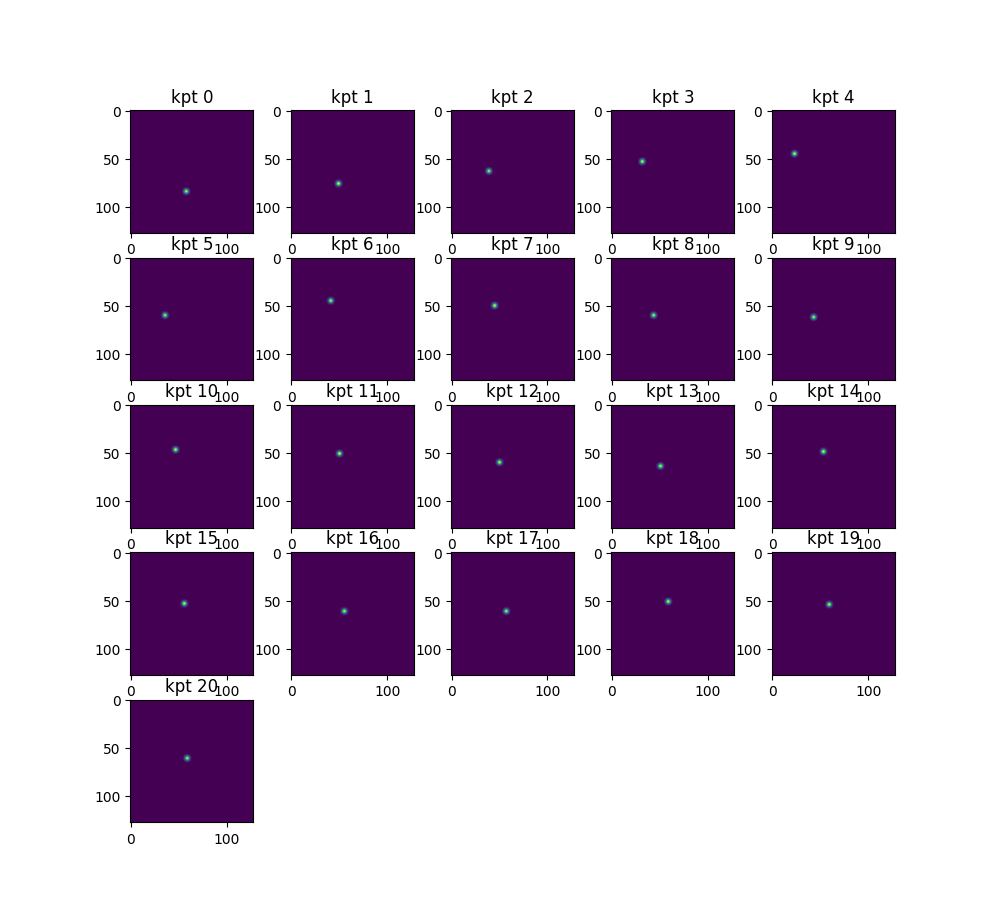
\includegraphics[width=250px]{assets/hand_heatmap_annotation.png}
            \caption{Pose 2D}
            \label{fig:hand_heatmap_annotation}
        \end{subfigure}
        \begin{subfigure}[b]{0.45\textwidth}
            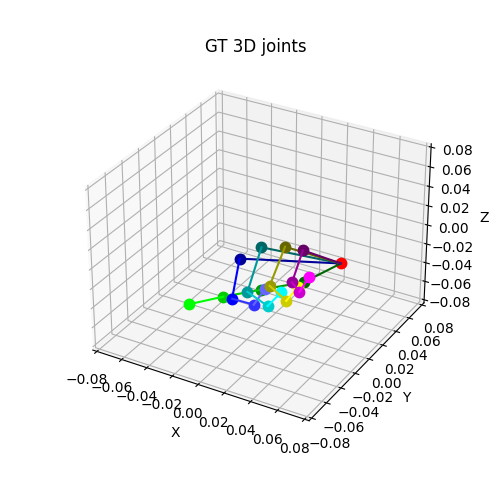
\includegraphics[width=200px]{assets/hand_pose_annotation.png}
            \caption{Pose 3D}
            \label{fig:hand_pose_annotation}
        \end{subfigure}
	    \caption{Pose Annotation}
	    \label{fig:hand_annnotation}        
    \end{center}
\end{figure}

\noindent
The IoU loss function is applied on the predicted heat maps to supervise the Pose 2D Estimator to learn the ground truth 2D heat maps \cite{olha}. The equation to compute the IoU loss is given in Equation \ref{eq:chernytska_iou_loss} \cite{olha}. The IoU measures the overlaps between the heatmaps for continuous values as shown in Equation \ref{eq:chernytska_iou}. The IoU loss is a value in the range from 0 to 1. A value close to 1 means the predicted matches the ground truth heatmaps and vice-versa. False negative is penalized in the Equation \ref{eq:chernytska_iou_intersection}, while false positive is penalized in the second term of Equation \ref{eq:chernytska_iou_union}.
\begin{equation}
L_{IoU} = 1 - IoU \label{eq:chernytska_iou_loss}
\end{equation}
\begin{equation}
IoU = \frac{I}{U} \label{eq:chernytska_iou}
\end{equation}
\begin{equation}
I = \sum_{i} (y_{pred,i} * y_{true,i}) \label{eq:chernytska_iou_intersection}
\end{equation}
\begin{equation}
U = \sum_{i} (y_{pred,i} * y_{pred,i}) + \sum_{i} (y_{true,i} * y_{true,i}) - \sum_{i} (y_{pred,i} * y_{true,i}) \label{eq:chernytska_iou_union}
\end{equation}
\noindent
The MSE loss function is applied on the predicted 3D poses to supervise the Pose 3D Regressor to learn the ground truth 3D poses \cite{semgcn, poseestimationreview}. The equation to compute the MSE loss is given in Equation \ref{eq:joint_positions_mse} \cite{semgcn, poseestimationreview}. The model treats the 3D poses as a regression tasks. A small loss indicates the predicted 3D poses matches the ground truth.
\begin{equation}
L_{mse} = \sum_{i} (P_{pred,i} - P_{true,i})^{2}\label{eq:joint_positions_mse}
\end{equation}
\noindent
The MSE loss function can also be applied on the predicted 3D bone vector to supervise the Pose 3D Regressor to learn the ground truth 3D bone vector \cite{semgcn}. The bone vector is computed by subtracting the positions of two 3D keypoints. The bone vector provides information on the direction and bone length that can help the model learn better. The equation to compute the MSE loss is given in Equation \ref{eq:bone_vector_mse} \cite{semgcn}. A small loss indicates the predicted 3D bone vectors matches the ground truth.
\begin{equation}
L_{mse} = \sum_{i} (B_{pred,i} - B_{true,i})^{2}\label{eq:bone_vector_mse}
\end{equation}


\newpage
\subsection{Robotic Arm Setup}
\noindent
MyCobot is setup to teleoperate via gestures from pose estimation on RGB images. Figure \ref{fig:robotic_arm_setup} shows the setup of the robotic arm in simulation on the left and in the real world on the right \cite{mycobot}. Unity3D is used for simulation \cite{unity3d}. The URDF of MyCobot is modified to include the gripper.

\begin{figure}[ht]
    \begin{center}
        \begin{subfigure}[b]{0.40\textwidth}
            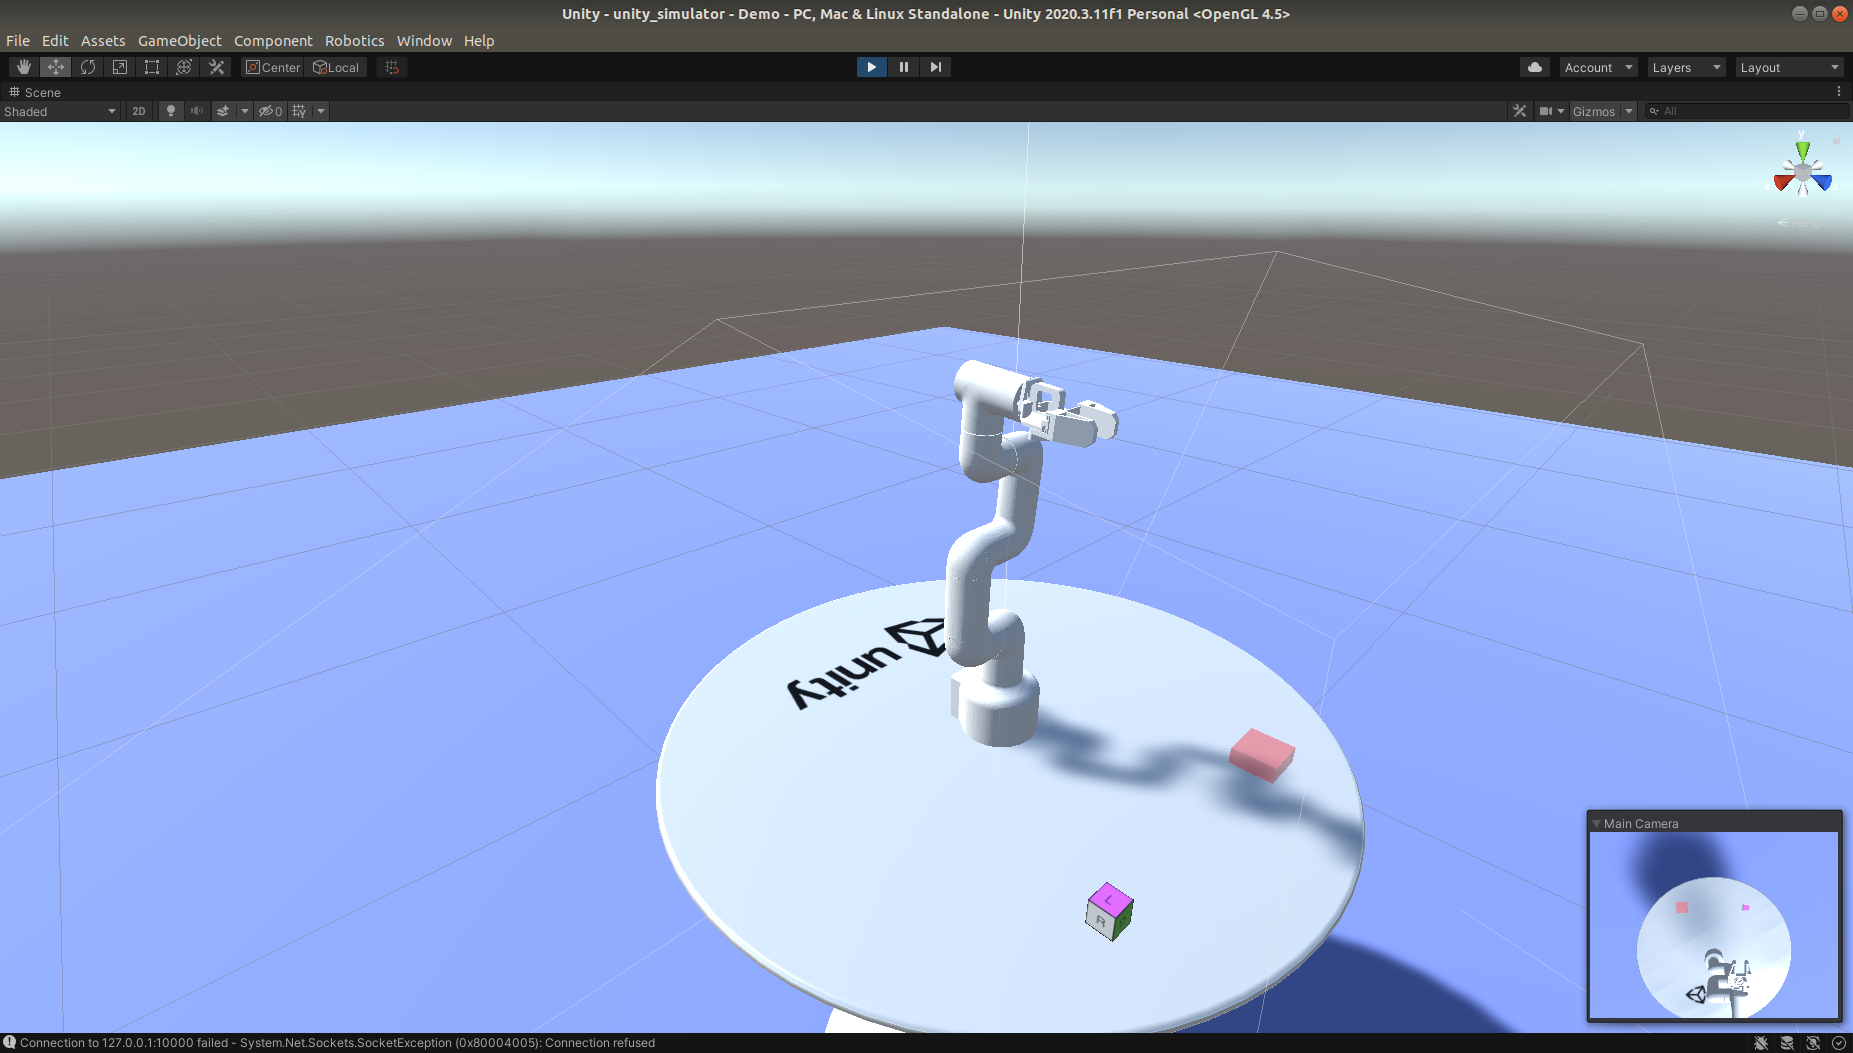
\includegraphics[width=180px]{assets/simulation_robot.png}
            \caption{Simulated Robot}
            \label{fig:simulated_robot}
        \end{subfigure}
        \begin{subfigure}[b]{0.22\textwidth}
            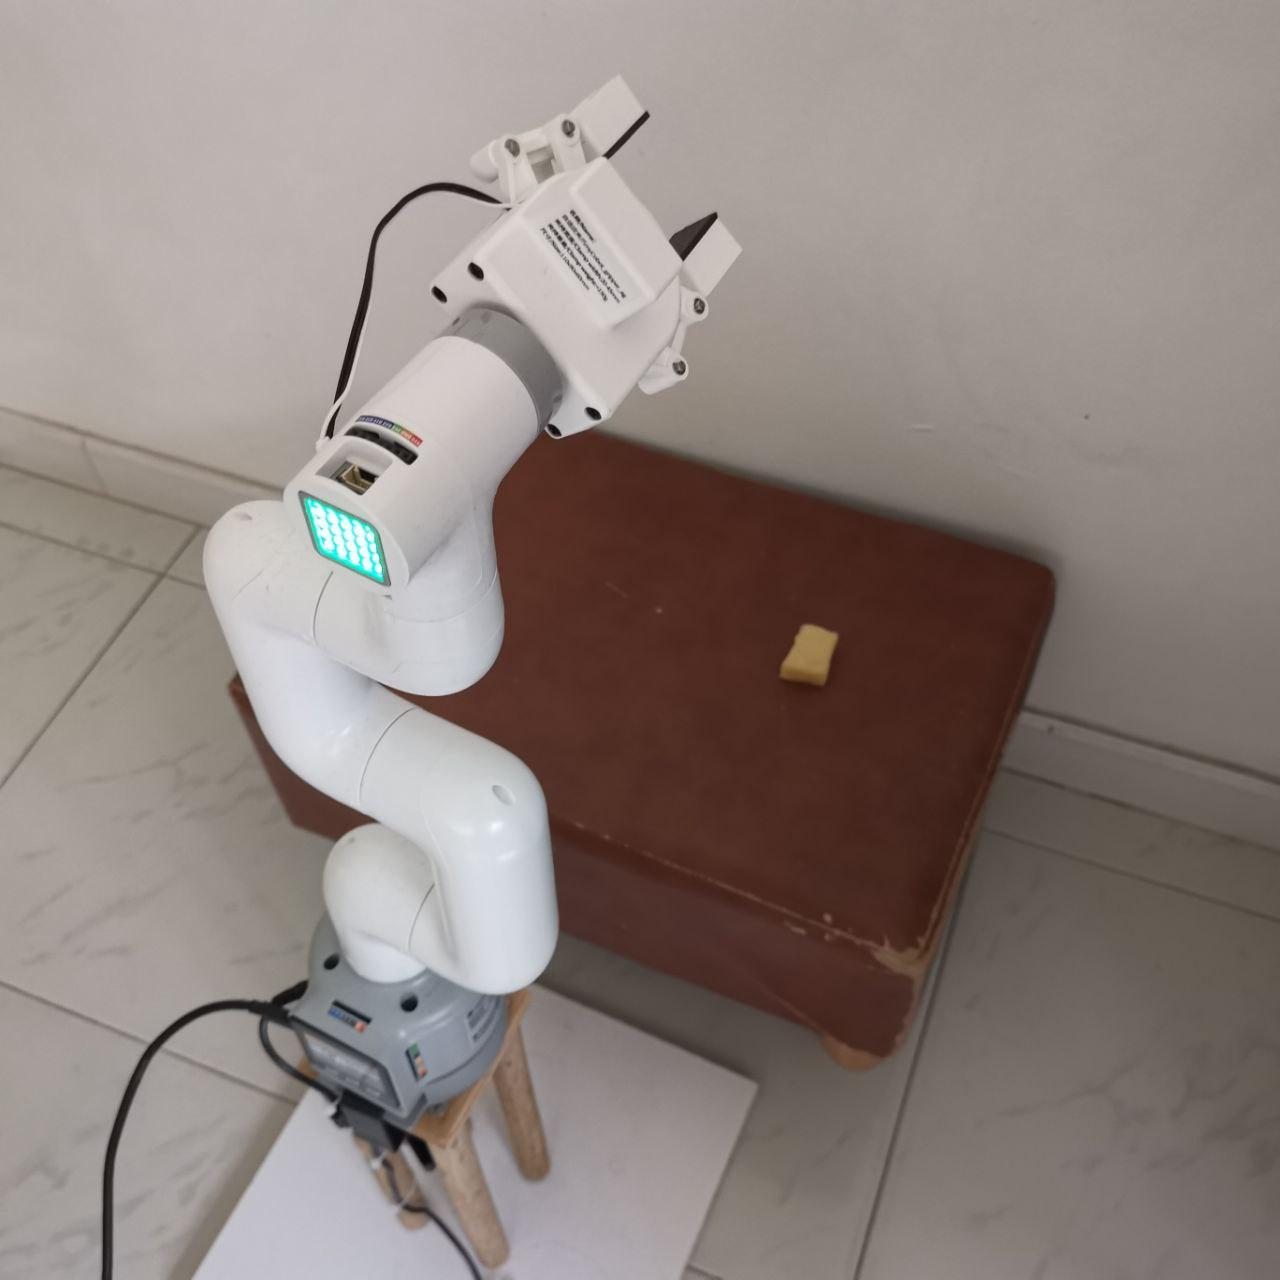
\includegraphics[width=100px]{assets/physical_robot.jpg}
            \caption{Physical Robot}
            \label{fig:physical_robot}
        \end{subfigure}
	    \caption{Robotic Arm Setup}
	    \label{fig:robotic_arm_setup}        
    \end{center}
\end{figure}
\noindent
ROS is used to modularise the robot development into subsystems, namely perception, navigation, and controller, as shown in Figure \ref{fig:ros_setup}. The Pose node extracts 3D poses from RGB images and publishes the pose. The Joints node publishes the current robot joints. The Controller node subscribes and receives the current robot joints and 3D poses. The Controller node also computes the start pose and end pose. The Trajectory Planner Service node plans the trajectory from start to end pose, while the Robot Motion Action Server node executes the trajectory to move the real robot and simulated robot.

\begin{figure}[ht]
	\begin{center}
		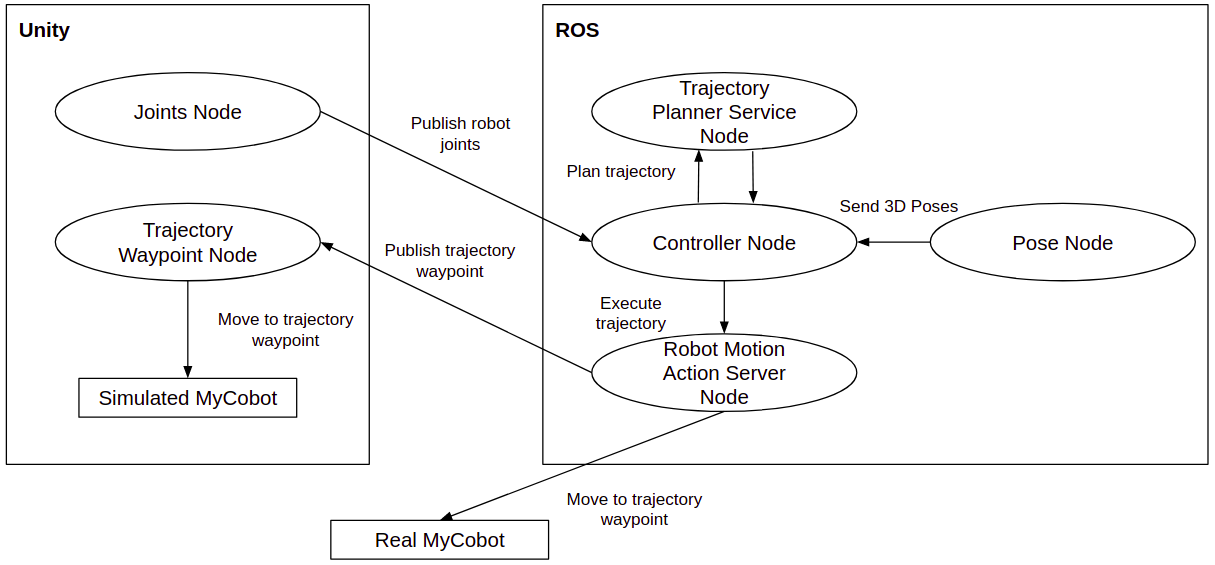
\includegraphics[width=300px]{assets/ros_setup.png}
		\caption{ROS Setup}
		\label{fig:ros_setup}
	\end{center}
\end{figure}
